%!TEX root = ../crimson_throne_book_main.tex
% 2016-05-21
The new Gray Maidens in the shrine to Irori do not only prove highly resistant to Quint's mind-affecting tricks, they also possess superior fighting skills. One of them challenges Balian and hits him extra hard, while her colleague makes her sword burn with black flames which bite at the ranger. Moreover, the two women fight in perfect unison, putting up a shield wall when the get attacked. Balian also finds that his special sense to fight 'humans' does not kick in when he faces these guards; his new sword's holy damage on the other hand flares up when his swings connect. With Spyder blocking off the third of these special maidens, Sjo and Quint are left with the two guards they encountered initially. These girls are definitely of a different kind than the three new Maidens, more within the limits of what you'd expect a Gray Maiden to be: human soldiers who possess some skill at battle, but who are by no means superwomen. This gives our friends the chance to cast some spells first: Sjo mumbles a {\itshape prayer} , while Quint enhances the party with  {\itshape haste} and starts up a  {\itshape satire} performance to debuff the enemy. Puk tumbles behind one of the super maidens, but sees his first stab deflected by her neighbor's shield. When he manages to get a cut in, he also finds that his tiny blades are partially resisted. Balian exchanges more blows with the supermaidens and is happy to learn that Sjo's magic of  {\itshape shield other} gives him much more staying power. He delivers a tremendous critical blow to the maiden on his left, just as Puk's many vicious slices take down the woman on his right. When the halfling delivers the final blow, the creature inside the elegant full plate splashes out in one huge burst of blood. The various pieces of her armor drop on the floor, soaked in red fluid \ldots but no body remains. This brings back memories. The party recalls Dame Nesia, the naked girl they found in the streets, who had lost any and all recollection of who she was or where she came from. As it turned out, the girl was some kind of blood simulacrum or blood clone. Balian suspects that these women are the same, albeit of a perfected nature. Sjo, who is badly hurt from taking half of Balian's damage, heals himself as Quint tries out his new rapier's powers on one of the ordinary maidens. The weapon's {\itshape inspire} ability allows him to use his bardic performance to enhance his swings with his charisma rather than his strength, making the bard a more formidable fighter in melee. Just when the companions seem to be getting the upper hand, the door ahead swings open and three more maidens join the fray, two of which fight like twins again. The third acts as somewhat of a tactician: she can guide her fellow soldiers in battle. Sjo recognizes a good opportunity when he sees one: the new and old opponents are all on the far side of the room, with only Puk in their midst. A perfect chance for a fireball! The explosion tears through the enemy, while the little halfling rogue manages to evade all the flames, laughing as another clone bursts out in a splash of blood. \hyperref[fig:Facing-the-Grey-Maidens-in-House-Leroung-610270843]{ His joy is quickly suppressed, however, when a red skinned devil appears behind the fresh forces, in the next hall, with Lady Eliasia Leroung in his clutches. } {\itshape``There they are, milady, your rebel friend! I knew they would show up! I knew it}'', the creature cackles, just before slicing his knife across Lady Leroung's throat. Her dead body drops to the floor. Quint is furious and shouts out threats to the murderer: {\itshape``You filthy leprechaun, you're gonna wish you'd never left Hell!}'' \\

\begin{figure}[h]
	\centering
	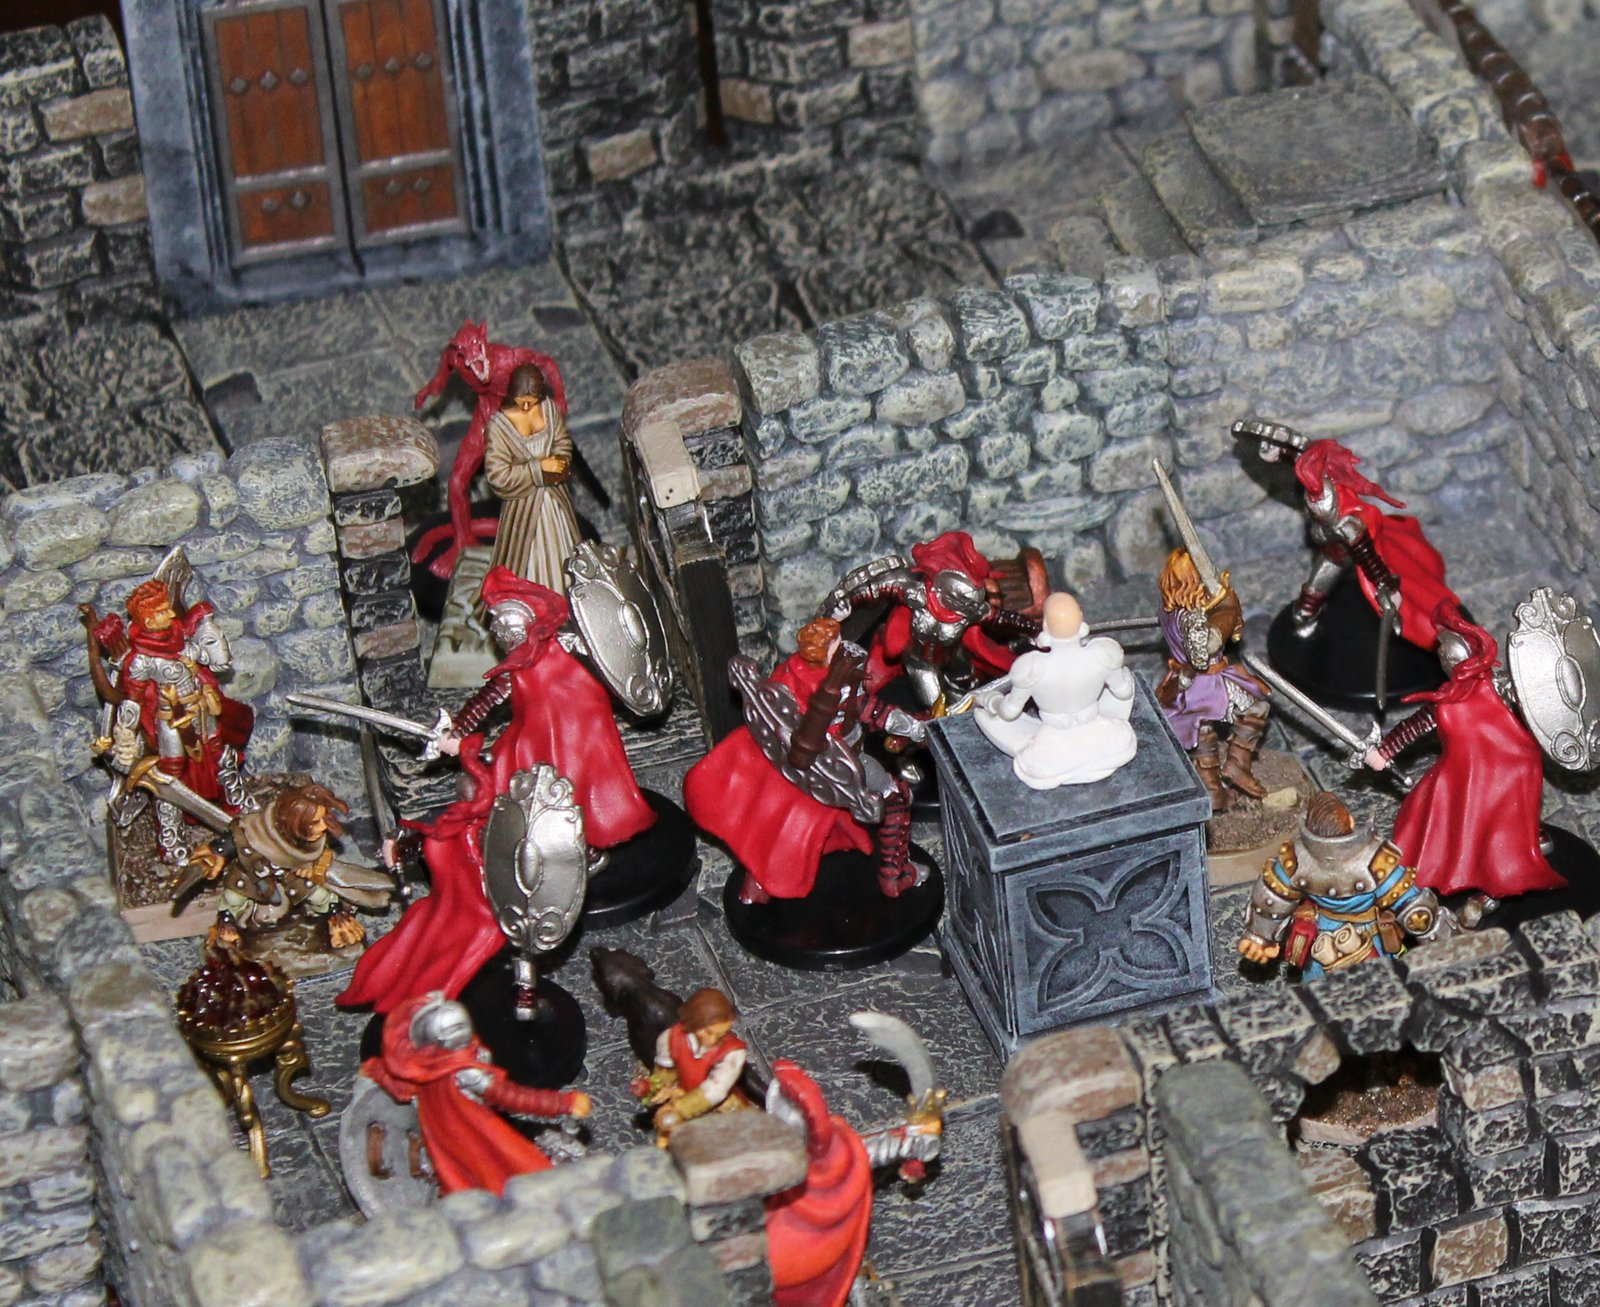
\includegraphics[width=0.39\textwidth]{images/Facing-the-Grey-Maidens-in-House-Leroung-610270843.jpg}
	\caption{Facing the Grey Maidens in House Leroung}
	\label{fig:Facing-the-Grey-Maidens-in-House-Leroung-610270843}
\end{figure}

In the meantime Puk and Balian take out another blood clone, Sjo continues healing and Quint cuts down one of the 'normal' Maidens. The devil zaps behind Sjo, but cannot do much damage before falling to Quint's wild attacks. The bard even makes sure the creature is truly defeated, by stabbing the corpse through the neck once more. Balian and Puk's efficiency takes care of the rest: two more blood clones and two human Gray Maidens bite the dust. One of these real maidens is still bleeding and Sjo makes sure she survives by stabilizing her. The victory does not grant joy, however, since Lady Eliasia lies truly dead and her children now run down the stairs to mourn her loss. Christina Leroung, her eldest daughter, is enraged at the companions. She lashes out at Quint for invading her home and getting her mother killed. When Balian mutters something about a possible resurrection she starts hitting him. This was an assassin devil, its victims cannot be brought back! She is also desperate about her family's future. Where should they go now? They will certainly be punished for this! The noblewoman keeps slapping Balian frantically, until he grabs her in a big bear hug to calm her down. Her sisters, Siri and Aisha (the opera star) and her aunt Sirtane (the alchemy professor) kneel down by Eliasia's body. Aisha and Siri are crying with great despair over their dead mother, while Sirtane does her best to whisper words of comfort. Cyril Fordyce, Eliasia's husband, the history professor and editor of the Herald, is staring with blind apathy.\\

Quint whisper some apologies, but Sirtane take shim to the next room to talk to him, as she is the only one who is in control of her emotions at the moment. Quint explains why they were here, they need to locate an ancient Shoanti grave somewhere under Korvosa. The tomb holds the corpse of a shaman who fought the evil that has now taken hold of Queen Ileosa. If they want to face her, they will need the shaman's aid. They were hoping to find clues in the library as to where the tomb might be situated. Sirtane understands and takes Quint to the 'history' room in the library, selecting a good number of books that the bard tucks away in his {\itshape bag of holding} . \hyperref[fig:Imps-in-House-Leroung-610269783]{ She also reveals that the library section on the 'planes' has been overrun by devils, imps, who are destroying a lot of the books. } Still the companions deem it unwise to attack \hyperref[fig:Fenryll-imp-in-House-Leroung-610270410]{ the critters; if one } escapes it could warn the enemy of the party's involvement and bring down hell on them, both in a figurative and literal sense. \hyperref[fig:Printing-press-in-House-Leroung-610271575]{ Quint and Balian also take a peek in the printing room } , where Ileosa's new seneschal Togomor has already been preparing the next issue of the Korvosan Herald, an edition that lauds the queen's efforts to save the city and serves as royal propaganda. \\

\begin{figure}[h]
	\centering
	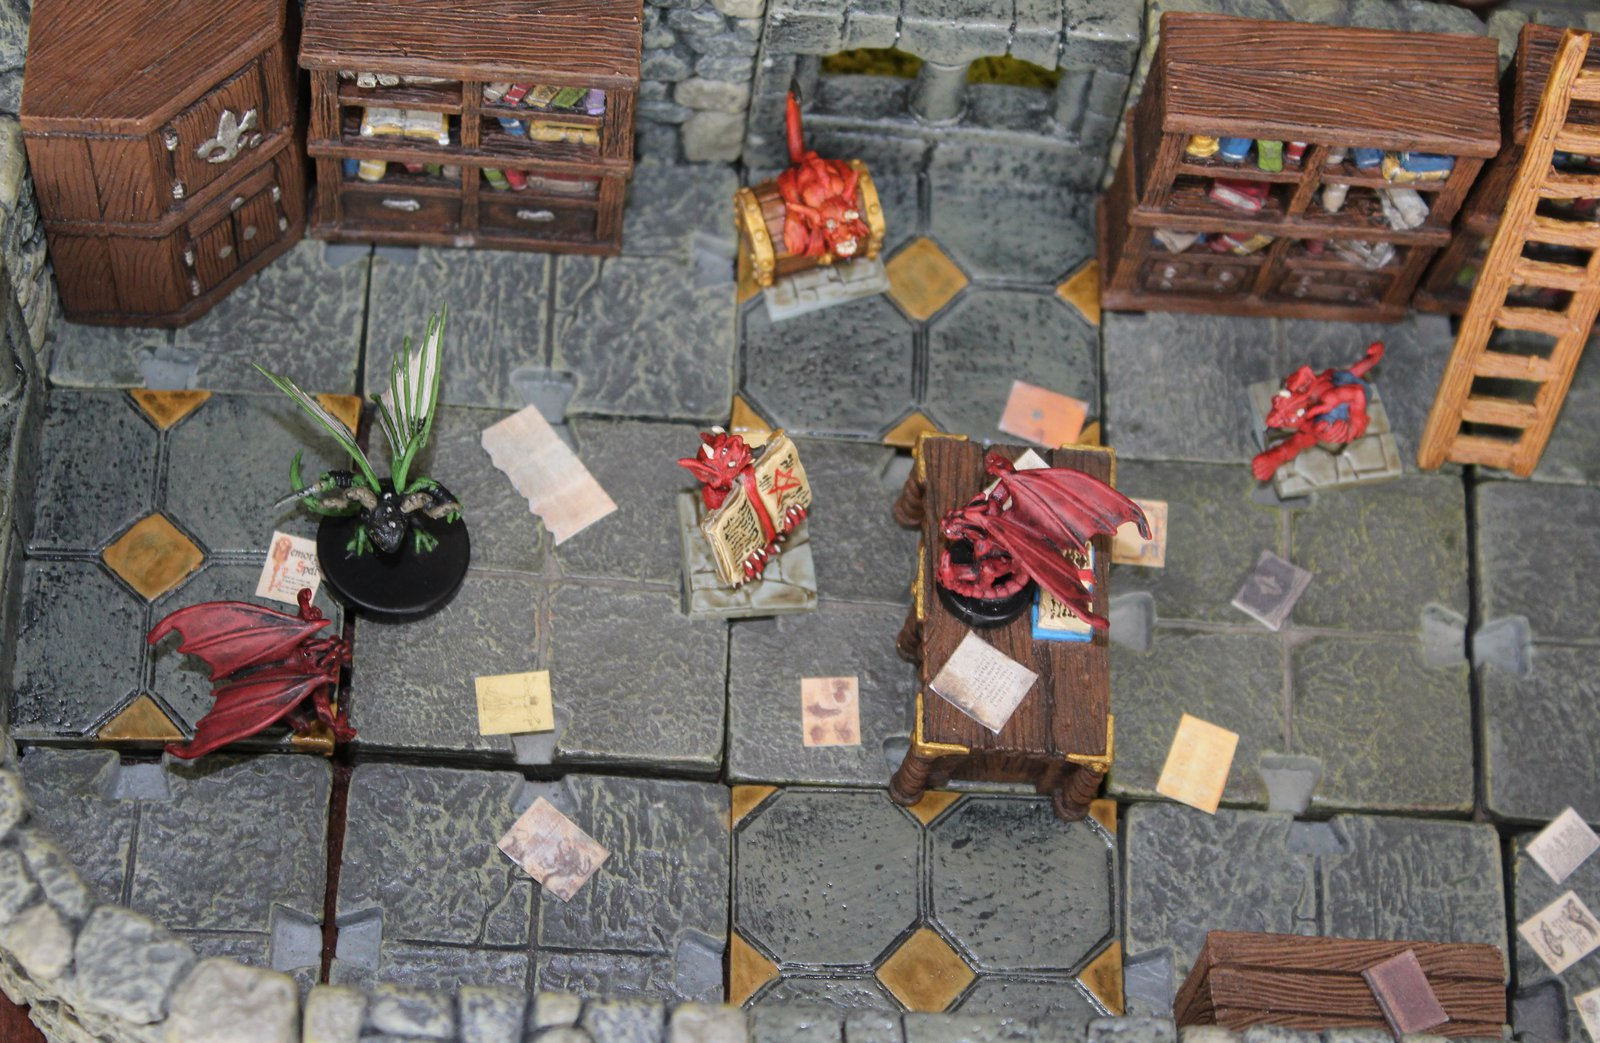
\includegraphics[width=0.39\textwidth]{images/Imps-in-House-Leroung-610269783.jpg}
	\caption{Imps in House Leroung}
	\label{fig:Imps-in-House-Leroung-610269783}
\end{figure}

\begin{figure}[h]
	\centering
	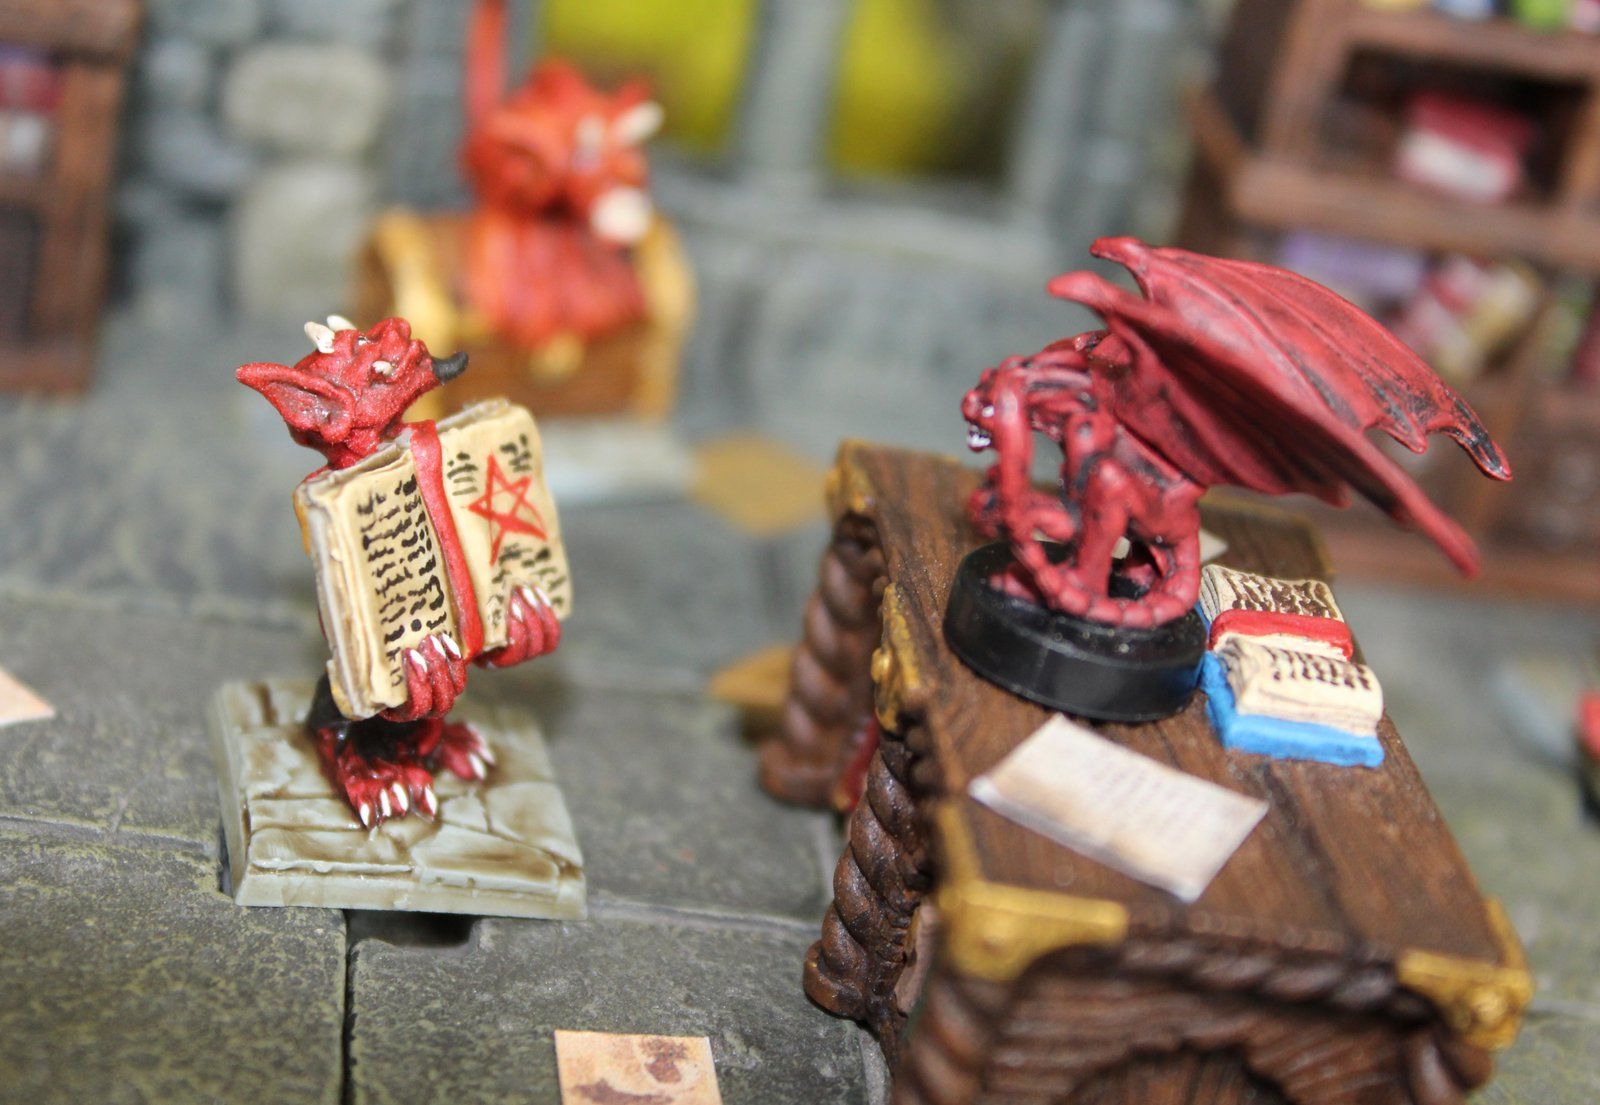
\includegraphics[width=0.39\textwidth]{images/Fenryll-imp-in-House-Leroung-610270410.jpg}
	\caption{Fenryll imp in House Leroung}
	\label{fig:Fenryll-imp-in-House-Leroung-610270410}
\end{figure}

\begin{figure}[h]
	\centering
	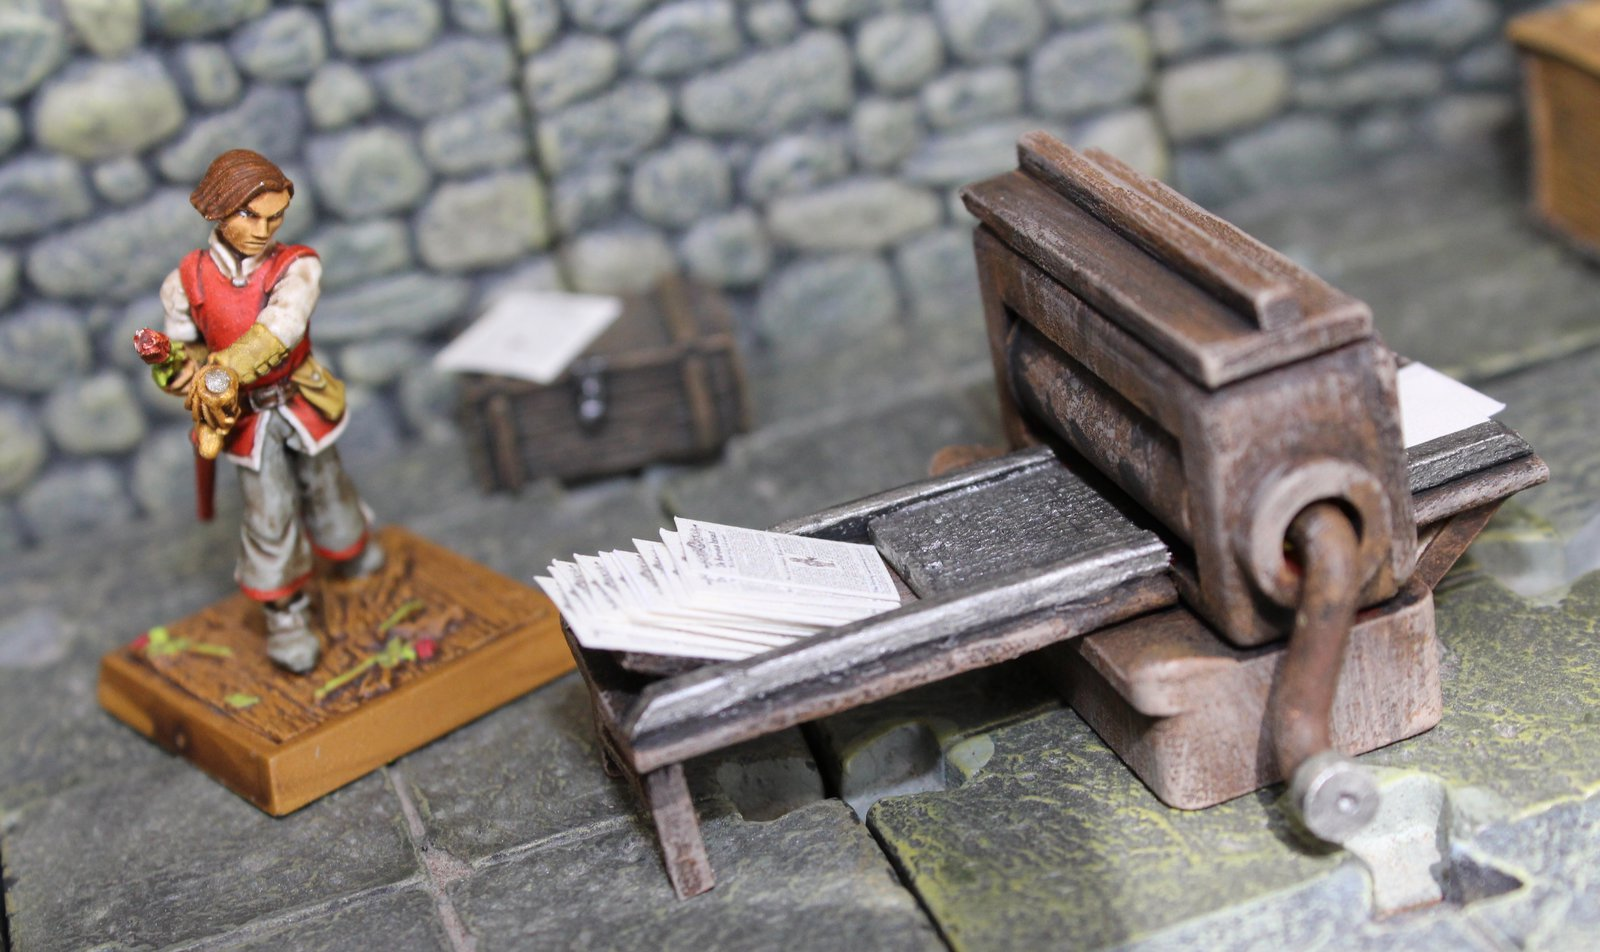
\includegraphics[width=0.39\textwidth]{images/Printing-press-in-House-Leroung-610271575.jpg}
	\caption{Printing press in House Leroung}
	\label{fig:Printing-press-in-House-Leroung-610271575}
\end{figure}

The companions decide to hide the Leroung family in the abandoned fishery that used to be to Gaedran Lamm's hideout. It is nearby and safe. They travel there under the cloak of invisibility, taking the corpse of Lady Eliasia with them. Afterwards they return to the Leroung residence to interrogate the surviving Gray Maiden. She seems to be one of the soldiers who came from Cheliax a few months ago. She sees no evil in working with devils, as these creatures are summoned to serve, not to command. When Quint gets mad at her for being blind to her malevolent acts, she returns the argument by calling him a rebel who refuses to accept the rightful ruler and as such being the cause of all this unpleasantness. Quint's anger gets the best of him: he draws his rapier and runs the woman through. His hope for finding redeemable Gray Maidens diminishes again, although he realizes that there must still be several women in their numbers who started out as good, normal Korvosans and who might only be misguided. Still, the uniforms and masks make it almost impossible to distinguish  between the soldiers. How will he be able to tell who can still be saved and who deserves to die?\\

